\documentclass[a4paper,11pt,hidelinks]{scrartcl}

\usepackage[ngerman]{babel}
\usepackage{graphicx}
\usepackage{url}
\usepackage{listings}
\usepackage{fontspec}
    \setmainfont{Vollkorn}
    \setsansfont{Lato}
    \setmonofont{Inconsolata}

\renewcommand{\baselinestretch}{1.25}
\pagestyle{headings}

\newcommand{\imgref}[1]{{Abbildung \ref{#1}, Seite \pageref{#1}}}

\begin{document}

\author{Patrick Bucher}
\title{v13r g3w1nn7}
\subtitle{Gamedesign-Portfolio: Vier Gewinnt für Sysadmins}
\date{\today}
\maketitle
\thispagestyle{empty}

\begin{center}
    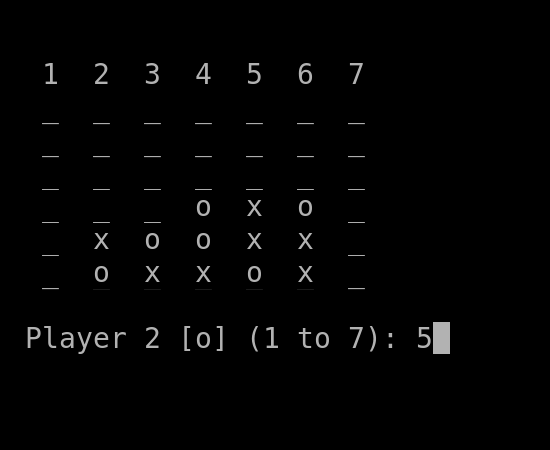
\includegraphics[width=0.5\linewidth]{pics/title.png}
\end{center}
%\newpage

\section*{Abstract}
Bla bla bla...
\newpage

\tableofcontents
\newpage

\section{Erste Iteration: Zieldefinition und Konzept}

Systemadministratoren (kurz: Sysadmins) haben es nicht einfach zu Zeiten der Corona-Krise: Ins Home-Office verbannt sind sie teilweise ihrer letzten sozialen Kontakte beraubt, zumal \textit{Star Wars}-Conventions und andere Veranstaltungen für Nerds alle abgesagt worden sind ‒ und dies auf eine lange Zeit hinaus. Als kleinen Trost sollen sie ein kleines Computerspiel bekommen, das im Rahmen dieses Projekts konzipiert und entwickelt wird. Dabei handelt es sich um eine erweiterte Version des Spiels «Vier Gewinnt».\footnote{\url{https://de.wikipedia.org/wiki/Vier_gewinnt}}

Sysadmins haben spezielle Bedürfnisse.\footnote{Als Sysadmin werden im Rahmen der vorliegenden Arbeit nur die Mitglieder der höchsten Kaste bezeichnet ‒ die Unix-Systemadministratoren. Auf die Bedürfnisse der Angehörigen tieferer Kasten soll hier nicht eingegangen werden.} Das herkömmliche «Vier Gewinnt» ist ihnen zu langweilig, zumal sie sämtliche Speilverläufe schon längst nachtsüber auf einem ihrer High-End-Server durchgerechnet haben. Zudem ist ihnen nach Spielende das lästige Sortieren der Steine nach Farben, das beim «Vier Gewinnt» im Meatspace nötig ist, ein Graus, zumal Sysadmins solche mechanischen Abläufe lieber automatisieren. Ausserdem lassen sich die Spielverläufe beim physischen Spiel nur sehr umständlich und schlecht maschinenlesbar festhalten, etwa mittels Fotokamera.

\begin{figure}
    \centering
    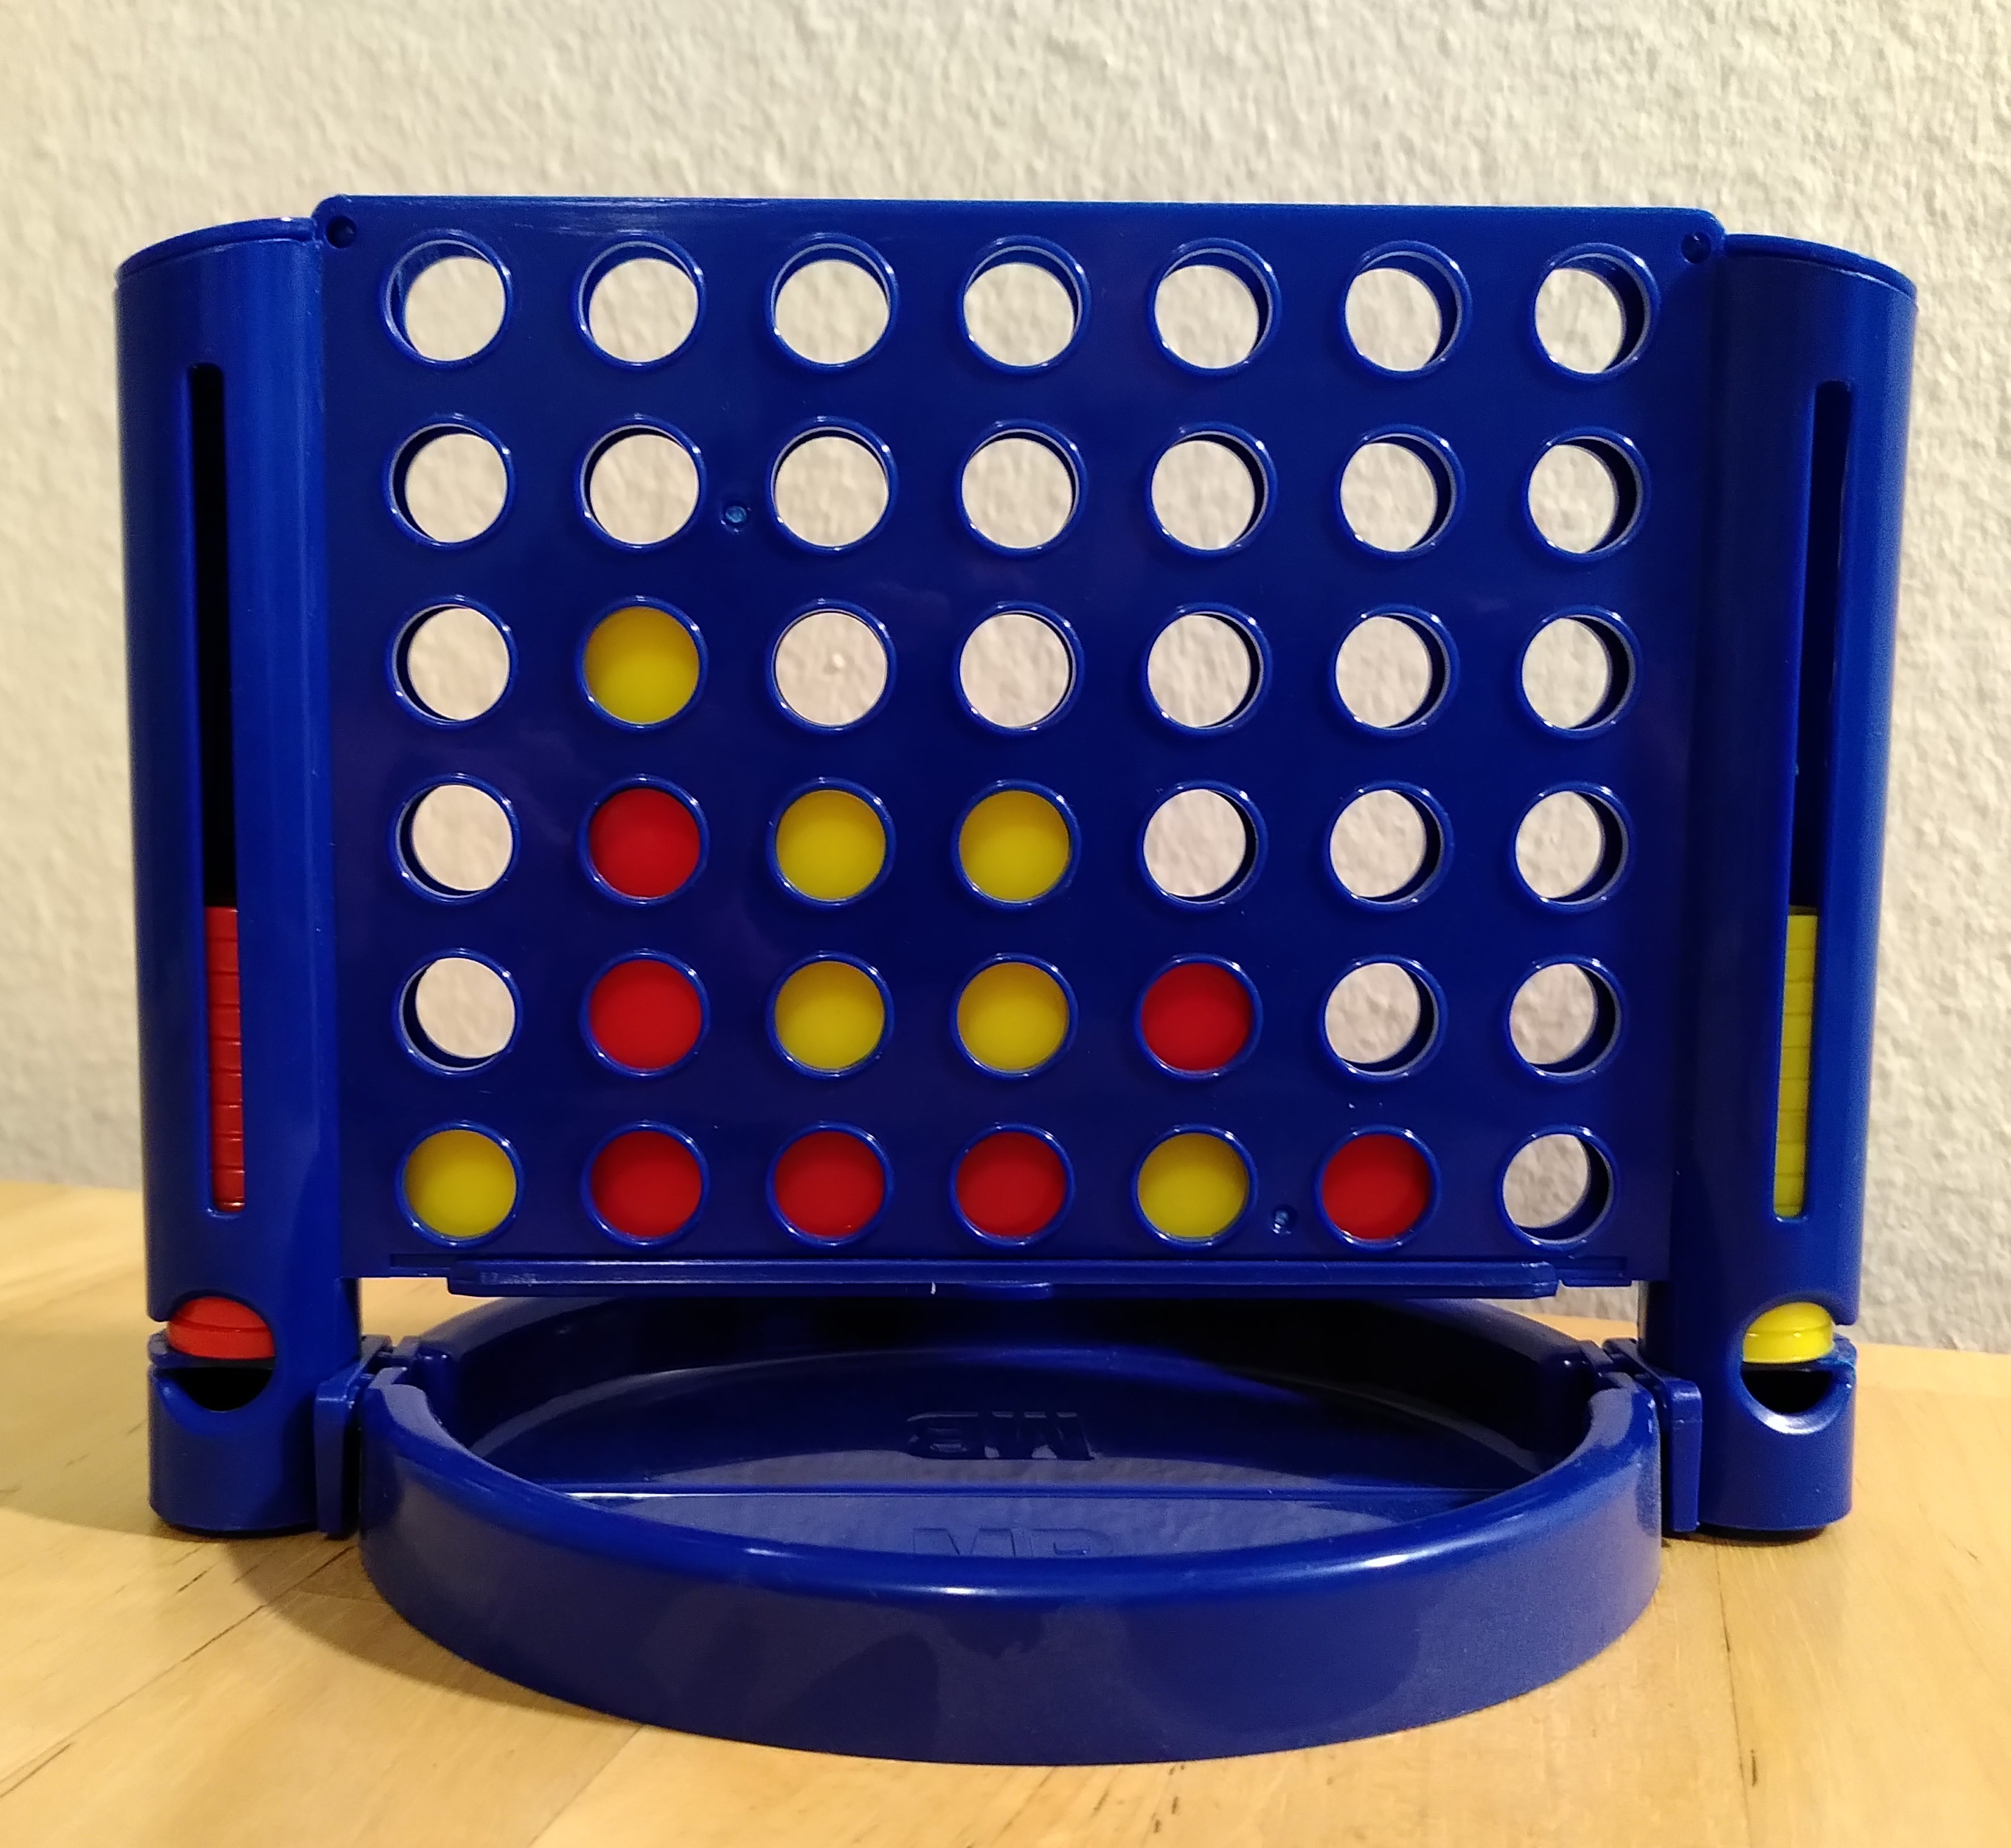
\includegraphics[width=0.7\linewidth]{pics/vier-gewinnt.jpg}
    \caption{Das klassische «Vier Gewinnt» (\textit{Meatspace}-Version). Die grellen Farben der VGA-Palette überfordern das auf die monochrome Bildschirmdarstellung optimierte Auge eines Sysadmins. Das analoge Einwerfen der Steine in die Schächte weckt traumatische Erinnerungen an die Handhabung einer Computermaus.}
\end{figure}

«Vier Gewinnt» wäre viel besser, wenn man es auf der Kommandozeile spielen könnte! Dies hätte folgende Vorteile gegenüber der herkömmlichen Meatspace-Version:

\begin{enumerate}
    \item Das Spiel könnte während der Arbeitszeit gespielt werden, ohne dass der gelegentlich vorbei- und in den Bildschirm schauende Vorgesetzte diese Strategie der Arbeitsvermeidung als solche erkennen könnte. Schliesslich handelt es sich ja bloss um irgendwelche kryptisch anmutende Zeichen, die da auf dem Bildschirm zu sehen sind. Bestimmt hat der Sysadmin da einen Belegungsplan für Pins oder dergleichen auf dem Bildschirm, und selbstverständlich handelt es sich dabei um geistige Schwerstarbeit, die dem Arbeitgeber zugute kommt ‒ das verrät schon des Sysadmins angestrengter Gesichtsausdruck!
    \item Die Aufforderung der Geschäftsleitung, mehr zu kommunizieren und sich Probleme gemeinsam anzuschauen, könnte für weitere Arbeitsvermeidung ausgenutzt werden, indem sich zwei Sysadmins am gleichen Computer treffen, um dort «Vier Gewinnt» (bzw. \texttt{v13r g3w1nnt!!!11}) zu spielen. Die kryptisch anmutende Pin-Be\-le\-gung, die da für den Vorgesetzten auf dem Bildschirm zu sehen ist, schreit ja geradezu nach einer \textit{Pair Debugging Session}! So kann die Arbeitszeit weiter mit «Vier Gewinnt» vertrödelt werden, und die sozialen Kontakte der Firma werden dadurch noch weiter gestärkt ‒ ganz im Sinne der Geschäftsleitung!
    \item Da solche sozialen Interaktionen im Meatspace derzeit wegen \textit{Social Distancing} kaum denkbar sind, müsste das Spiel auch remote von zwei Sysadmins spielbar sein, ohne dass die Nerds der Softwareentwicklung das Spiel aufwändig umprogrammieren müssen. So könnten die Sysadmins das Spiel von zu Hause aus über eine gemeinsame Session mit \texttt{tmux} oder GNU \texttt{screen} gegeneinander spielen. Dies dürfte auch die VPN-Verbindung ins Büro nicht weiter beeinträchtigen, zumal diese schon durch BitTorrent-Downloads voll ausgelastet ist. Der Multiplayer-Modus wäre somit auch über eine serielle Verbindung möglich, die der erfahrene Sysadmin notfalls auch aus im Büro gestohlenen Büroklammern und aus abgerissenen Streifen seines Aluhuts herstellen könnte. Sollte der Bildschirm des Sysadmins unerwartet in die Brüche gehen, wäre das Spiel immer noch über einen Fernschreiber spielbar, der sich bei jedem guten Systemadmin im Keller finden lässt.\footnote{In der Regel hinter der Kiste mit den \textit{Star Trek}-Fanartikeln.}
    \item Die Spielverläufe können einfach in Textdateien\footnote{d.h. MIME-Type \texttt{text/html;charset=utf-8}, selbstverständlich ohne \textit{byte order mark} (BOM)} festgehalten werden. Das erleichtert die Diskussion über Spielstrategien auf dem Usenet und in IRC.
\end{enumerate}

Das klassische «Vier Gewinnt» müsste hierzu natürlich noch etwas interessanter ausgestaltet werden, sodass die Motivation der Sysadmins zumindest das Warten auf den nächsten Download auf den derzeit chronisch überlasteten Steam-Servern überdauert. Diese möglichen Verbesserungen sollen im Rahmen dieser Arbeit vorgeschlagen, umgesetzt und evaluiert werden.

\subsection{Zwei Tastaturen, eine Kommandozeile}

\newpage

\section{Zweite Iteration: Anwendung von Game-Design-Theorie}
\newpage

\begin{figure}
    \centering
    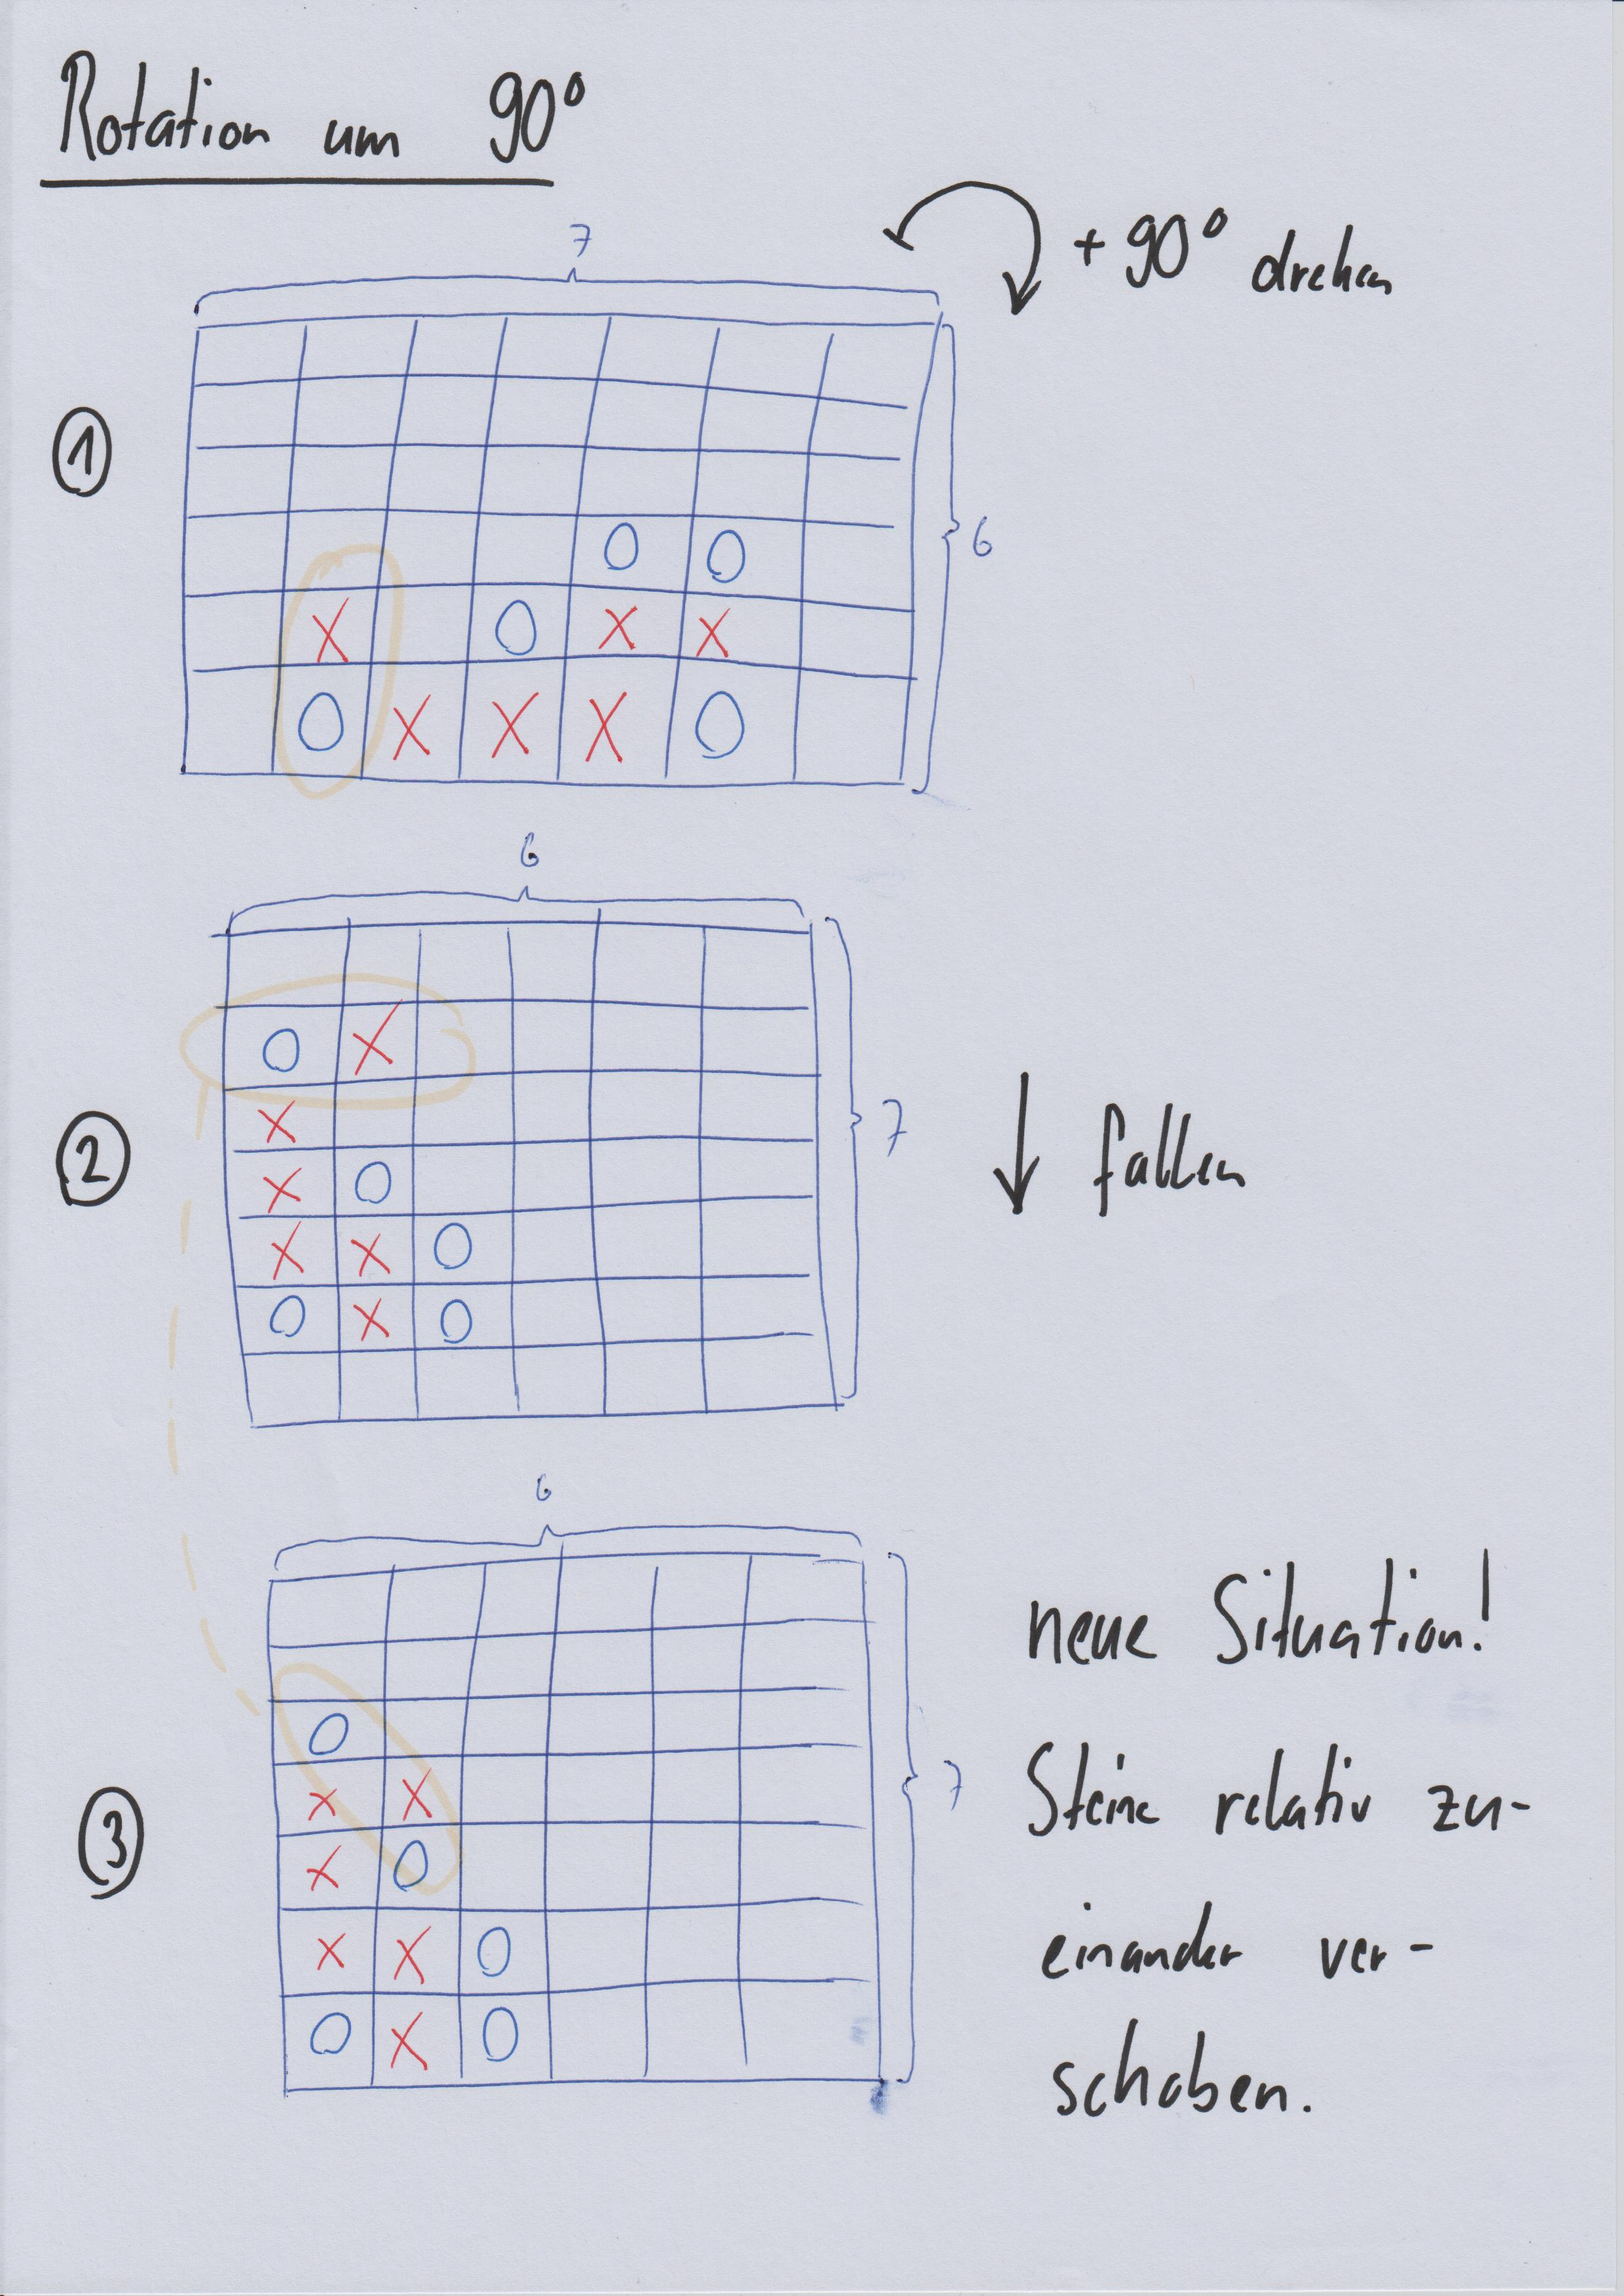
\includegraphics[width=0.7\linewidth]{pics/rotation-papier.jpg}
    \caption{Die Rotation um 90° als zusätzliche Spielmechanik. Das Spielgitter wird zunächst gedreht, anschliessend fallen die Steine nach unten. So entsteht eine neue Spielsituation, da sich manche Steine relativ zueinander bewegen.}
\end{figure}

\section{Dritte Iteration: Abschliessender Nutzertest und Reflexion}
\newpage

\listoffigures
\addcontentsline{toc}{section}{Abbildungsverzeichnis}

\end{document}
